


This chapter details the proposed framework and implementation. I start by giving an overview of the proposed framework, and then five crucial components in the framework are carefully explained: Deep Denoising Autoencoders on audio-visual modalities, Fisher Vector Encoding, Document Embedding on textual modality, Tree-based Feature Selection and Multi-Task Learning. 





\section{Overview}

Figure \ref{fig:pipeline} illustrates the framework of my proposed method for automatic Bipolar Disorder BD recognition. For acoustic modality, I extract 39-dimensional Mel-Frequency Cepstrum Coefficients (MFCCs)\footnotemark as the Low-Level Descriptors (LLDs) with OpenSMILE and for visual modality, I extract the 132-dimensional facial landmarks, 6-dimensional head pose, 6-dimensional eye gaze, and 35-dimensional Facial Action Units (FAUs) as the LLDs with OpenFace. To discover the correlation across audio-visual modalities and produce robust representations, I propose a Deep Denoising Autoencoder (DDAE) that learns a shared and joint representation on different number of modalities. More specifically, according to the number of modalities on which DDAEs are built, I define uni-DDAE, bi-DDAE, and multi-DDAE. Before feeding multimodal features into DDAE, features must be aligned on frame-level first to ensure they are extracted from the same time interval. I then compute the dynamic changes of the latent representations in DDAE as each representation is regarded as a specific movement of the subject. After computing the velocity ($1^{st}$-order derivative) and the acceleration ($2^{nd}$-order derivative) of the latent representations, the three features are concatenated as frame-level descriptors. Because the video clips vary in length, I encode the frame-level descriptors with a Fisher Vector (FV), a fixed-length descriptor on session-level, by fitting them into a Gaussian Mixture Model (GMM). To reduce redundancy and select the most discriminative feature set, a tree-based model is used for feature selection by evaluating the feature importance.


\begin{figure}[ht]
    \centering
    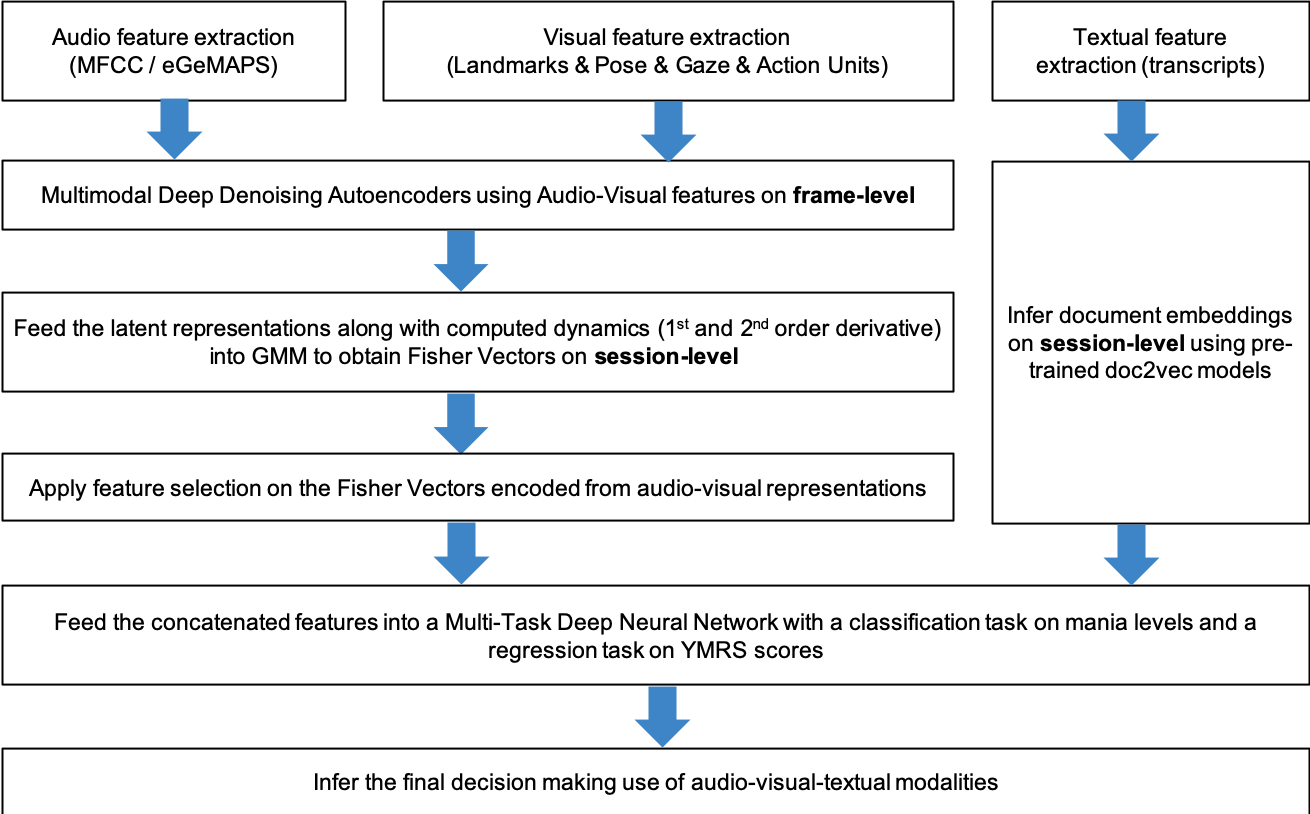
\includegraphics[width=13.5cm]{images/design/general_pipeline.png}
    \caption{Pipeline of the proposed framework that includes different learning architectures on different modalities}
    \label{fig:pipeline}
\end{figure}

On the other hand, I obtain the transcripts of video interviews and apply a document embedding model (doc2vec) to learn fixed-length representations of the transcripts on session-level. To boost the performance of the doc2vec model, the model is pre-trained on an additional Turkish corpus. 

With both fixed-length FVs on audio-visual modalities and fixed-length document embeddings on textual modality, a Multi-Task Deep Neural Network (MT-DNN) is built to handle the overfitting due to the limited size of the BD corpus. The MT-DNN is learned with a weighted loss from the ternary classification task of Mania Level and the regression task of Young Mania Rating Scale (YMRS). Furthermore, to address the imbalance between three classes, I duplicate the training instances of the minority class and apply Unweighted Average Recall (UAR) as my metric for evaluation. Finally, with the best-performing MT-DNN, the final decision on each video interview is inferred: depression, hypo-mania, or mania.


\footnotetext{The 39-dimensional MFCC features are obtained by appending additional 13 delta and 13 acceleration coefficients to the conventional 13-dimensional MFCC features.}









\section{Deep Denoising Autoencoders}
\label{sec:DDAE}

Autoencoders (AEs) are an unsupervised learning algorithm that learns a latent-space representation of given data with hidden layers constrained while reconstructing the data from the representation. The representations learnt from AEs generally have a lower dimensionality and have been proven effective as high-level features in the following classification tasks, which in many cases are competitive or even superior to the hand-engineered representations \cite{ng2011}. Autoencoders are composed of two parts: a) encoder, which compresses the input into a latent representation with the function $h=f(x)$, and b) decoder, which reconstructs the input from the latent representation with the function $r=g(h)$, as shown in Figure \ref{fig:unimodal_ae}. Therefore, autoencoders can be described by the function $g(f(x))=r$, and the reconstruction error $\parallel x-r \parallel ^ 2$ is minimized in the training processing. 

\begin{figure}[ht]
    \centering
    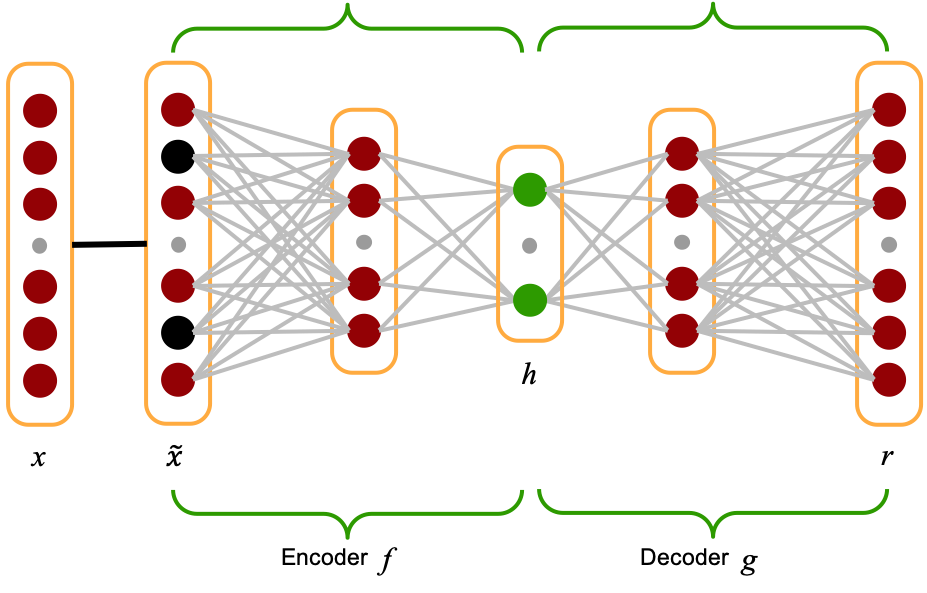
\includegraphics[height=6.5cm]{images/design/autoencoder.png}
    \caption{Schematic for Unimodal Deep Denoising Autoencoders}
    \label{fig:unimodal_ae}
\end{figure}


Autoencoders were first introduced as an approach to initialize the weights of neural networks \cite{ballard1987}, and because of the \textit{curse of dimensionality} \cite{bellman1966}, the low-dimensional hidden layers enable AEs to be commonly employed in feature engineering and representation learning \cite{charte2018}. Several variations of AEs have been developed with different constraints on the hidden layers, such as sparse AEs \cite{ng2011}, denoising AEs \cite{vincent2008}, and variational AEs \cite{kingma2013}. 

Denoising AEs, proposed by \cite{vincent2008}, stochastically corrupts part of the original input $x$ and reconstructs the original input $x$ with the corrupted version $\tilde{x}$. The noise can be of different forms, such as additive isotropic Gaussian noise and masking noise \cite{vincent2010}. The Gaussian noise $\tilde{x}$ is obtained with $\tilde{x}|x \sim \mathcal{x, \sigma^2,I}$ and the masking noise is calculated by forcing a fraction $v$ of the elements of input $x$ to 0. Although the Gaussian noise is reported to be the natural choice for real-valued inputs \cite{vincent2010}, I only consider the masking noise in the experiment as the Gaussian noise could introduce a small change in facial expressions, which could be interpreted as a misleading descriptor for the BD symptoms. The objective of denoising AEs accordingly becomes minimizing the reconstruction error $\parallel \tilde{x}-r \parallel ^ 2$. The denoising AEs are reported to produce representations that are robust to small irrelevant changes in the input.

With the development of multimedia data processing, a more recent learning architecture is introduced for feature fusion: the multi-modal AEs \cite{mangai2010}. Feature fusion aims to learn a shared representation cross modalities without redundant or irrelevant information, which is one of the biggest challenges in multi-modal data processing \cite{mangai2010}. In the work of \cite{hong2015}, authors aimed to perform multimodal fusion of 2D images and 3D human poses to obtain high-level representations. 
Inspired by \cite{vincent2008}, \cite{mangai2010}, and \cite{dibekliouglu2017}, I propose a series of 3-layer Deep Denoising Autoencoders (DDAEs) (i.e., DDAEs with 3 hidden layers) with different number of modalities to investigate the multimodal fusion in the BD detection task. 

\subsection{Unimodal Deep Denoising Autoencoders}

I first define the unimodal DDAEs on acoustic and visual features respectively as shown in Figure \ref{fig:unimodal_ae}, where features of one modality are fed into DDAEs to learn a compact-size representation after adding masking noise. This architecture is considered as a baseline for the following architectures as it does not discover the correlation across modalities. 

In many implementations of AEs, the binary cross-entropy (BCE) is set as the loss function, which measures the amount of information is preserved in the reconstruction compared to the original input \cite{de2005}. BCE is calculated with Equation \ref{eq:binarycrossentropy}, in which $x_k$ represents one node in the input layer and $r_k$ represents the corresponding node in the output layer. The input data must be therefore normalized to the range $[0,1]$ with the sigmoid activation function in the output layer. BCE could apply to binary-value image pixel intensities, such as MNIST dataset, because the range of original intensities lies in $[0, 255]$, but other features, like MFCC, rarely share the same range across the dataset and normalization could wrongly corrupt the correlation in features, thus hurting the extraction of emotion-related information. In my framework, instead, I define the loss function as the mean squared error (MSE) (Equation \ref{eq:mse}) with the linear activation function in the output layer and no normalization. The DDAEs are trained on minimizing the distance between reconstructed input and original input, and the reconstruction could be easily interpreted and visualized in the evaluation.

\begin{equation}
    J(x,r) = - \sum_{k=1}^d x_k \log(r_k) + (1-x_k) \log(1-r_k)
    \label{eq:binarycrossentropy}
\end{equation}

\begin{equation}
    J(x,r) = \frac{1}{N} \sum_{k=1}^d (x_k - r_k)^2
    \label{eq:mse}
\end{equation}


\begin{figure}[ht]
    \centering
    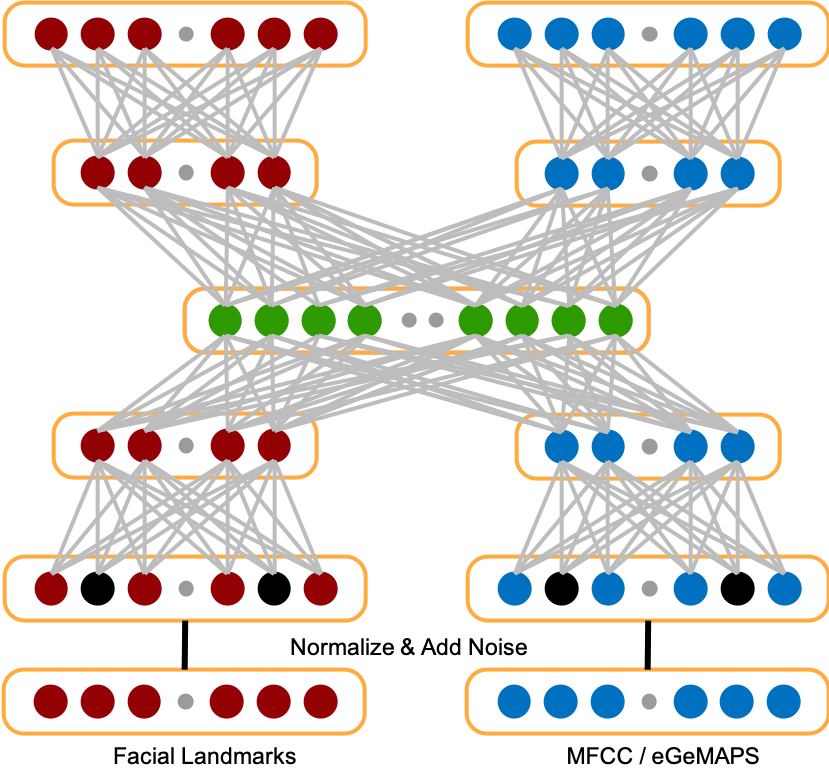
\includegraphics[height=7.5cm]{images/design/bimodal_ae.png}
    \caption{Schematic for Bimodal Deep Denoising Autoencoders (Different colours indicate different modalities)}
    \label{fig:bimodal_ae}
\end{figure}


\subsection{Bimodal Deep Denoising Autoencoders}

I continue to define the 3-layer bimodal DDAEs on acoustic and visual features altogether as displayed in Figure \ref{fig:bimodal_ae}. The acoustic features are Low-Level Descriptors (LLDs), either MFCC or eGeMAPS features, and the visual features in this architecture are set as facial landmarks whose dynamics have been proven useful in depression detection \cite{dibekliouglu2017}. As suggested in the work of \cite{ngiam2011}, two separate encoders are merged into one shared hidden layer after one hidden layer, which outputs the first-order representations. From the shared hidden layer, two modalities are then reconstructed via their decoders with the sum of MSE on both reconstructed inputs as the loss function. 
Acoustic and visual modalities need to be aligned beforehand to ensure they are within the same window \cite{ngiam2011}, and I concatenate 3 contiguous acoustic features as each input that has approximately the same duration as 1 visual feature. Because audio-visual modalities have different data formats and ranges, they are normalized and whitened separately.

\begin{figure}[ht]
    \centering
    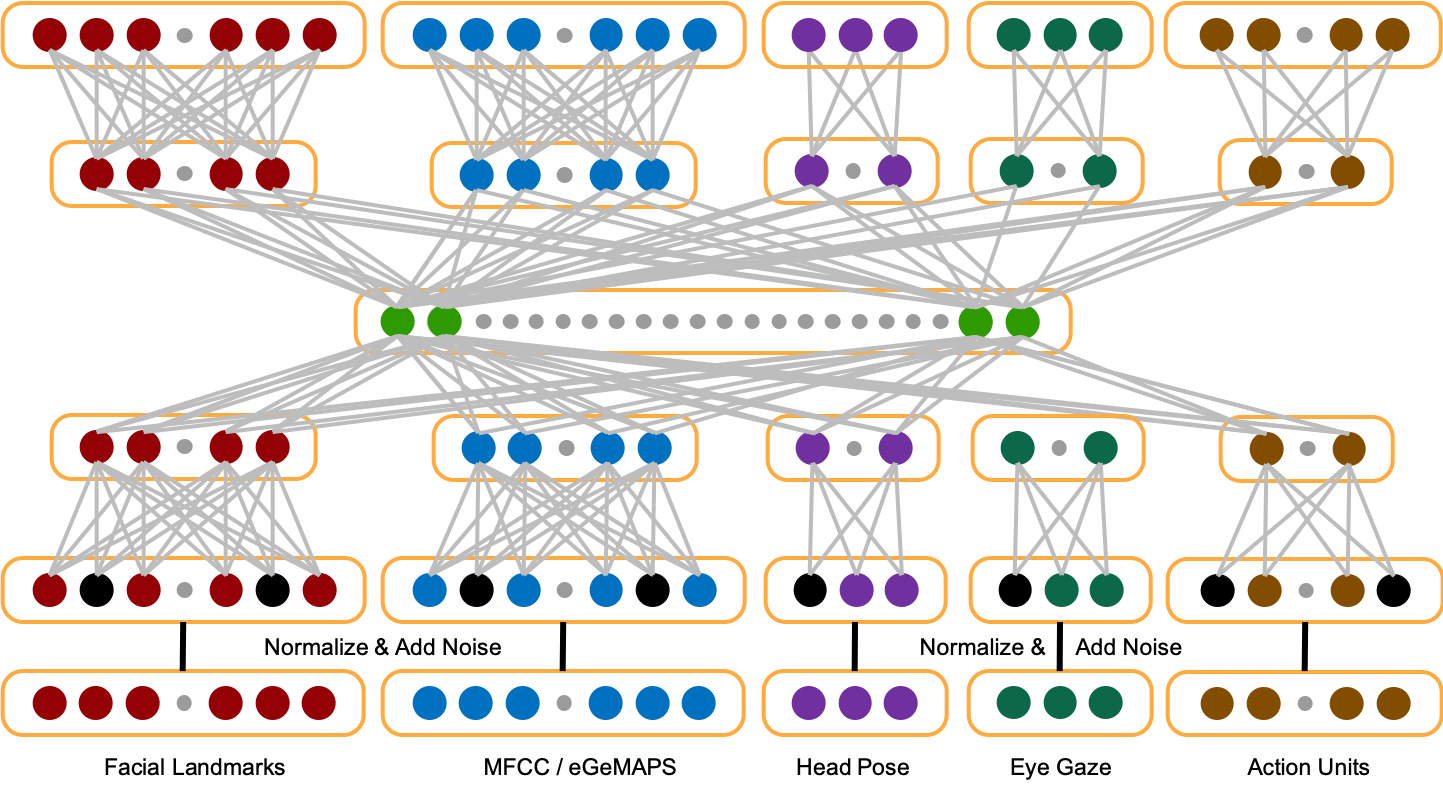
\includegraphics[height=7.5cm]{images/design/multimodal_ae.png}
    \caption{Schematic for Multimodal Deep Denoising Autoencoders (Different colours indicate different modalities)}
    \label{fig:multimodal_ae}
\end{figure}

\subsection{Multimodal Deep Denoising Autoencoders}

Given the importance of head pose, eye gaze, and action units in emotion recognition \cite{adams2015, ekman2013}, the 3-layer multimodal DDAEs are defined on a total of five modalities, namely facial landmarks, MFCC / eGeMAPS, head pose, eye gaze, and action units (shown in Figure \ref{fig:multimodal_ae}). Following the same design principle as the bimodal DDAEs, five modalities are merged into the shared representation layer with their ``mid-level" representation output by their first hidden layer, and masking noise is added to modalities individually. The reconstruction loss of each modalities is assigned with equal weights in the joint reconstruction loss function. 

\subsection{Implementation Details}

The list of investigated hyperparameters for all DDAEs is given in Table \ref{tab:param_DDAE}, in which the hidden ratio is defined as the ratio between two consecutive hidden layers, and for instance, with hidden ratio 0.5, the dimensions of all hidden layers would be $\{0.5d, 0.25d, 0.5d\}$ where $d$ represents the input dimensionality. In addition, I evaluate the denoising effect in DDAEs by setting different masking noise levels.


\begin{table}[ht]
    \centering
    \caption{Hyperparameter settings to investigate for DDAEs}
    \begin{tabular}{l|l}
        \Xhline{2\arrayrulewidth}
        Hyperparameter & Values \\
        \hline
        hidden ratio & \{0.4, 0.5\} \\
        noise level & \{0.1, 0.2, 0.4\} \\
        batch size & 1024 \\
        learning rate & 0.01 \\
        epochs & 100 \\
        \Xhline{2\arrayrulewidth}
    \end{tabular}
    \label{tab:param_DDAE}
\end{table}

The dimensions of all input modalities are listed in Table \ref{tab:dim_modality}. Because the shared representation is trained from only one acoustic features, either MFCC features or eGeMAPS features are input into bimodal DDAEs (Table \ref{fig:bimodal_ae}) and multimodal DDAEs (Table \ref{fig:multimodal_ae}). The sum of the input dimensions would thus be either 300 or 252, and the shared representation has four different dimensions with different hidden ratio settings (either 0.4 or 0.5), as shown in the last two row of Table \ref{tab:dim_modality}. The dimension of facial landmarks is obtained by $x$ and $y$ coordinates of 68 landmarks, while to acoustic features, dimensions of MFCC and eGeMAPS are multiplied with 3 because of the alignment of audio-visual modalities.

The training of DDAEs can be considered as the unsupervised feature learning, in which more data benefit the encoding of DDAEs \cite{ngiam2011}. All DDAEs are therefore trained with all available labelled (training set and development set) and unlabelled (test set) audio-visual data. 

\begin{table}[ht]
    \centering
    \caption{Dimension of all five modalities. The two dimensions of representations in the last two rows are based on the different hidden ratios, defined in \ref{tab:param_DDAE}}
    \begin{tabular}{l|l}
        \Xhline{2\arrayrulewidth}
        Modality & Dimension \\
        \hline
        Facial Landmarks & 136 ($68 \times 2$) \\
        MFCC features & 117 ($39 \times 3$) \\
        eGeMAPS features & 69 ($23 \times 3$) \\
        Head Pose & 6 \\
        Eye Gaze & 6 \\
        Action Units & 35 \\
        \hline
        Sum of input (MFCC) & 300 \\
        Sum of input (eGeMAPS) & 252 \\
        \hline
        Representation (MFCC) & 48 (0.4) / 75 (0.5) \\
        Representation (eGeMAPS) & 40 (0.4) / 63 (0.5) \\
        \Xhline{2\arrayrulewidth}
    \end{tabular}
    \label{tab:dim_modality}
\end{table}

\subsection{Computing Dynamics of Latent Representations}

After training, each DDAE (unimodal, bimodal, or multimodal) learns a presentation for the per-frame extracted features. These representations, however, only encode the static element of the input, such as locations of facial landmarks or loudness of audio signal, but without any temporary information. Following the ideas proposed in \cite{dibekliouglu2017}, I extend these representations with the dynamics. Considering DDAE-based representations as a matrix $H \in \mathcal{R}^{n \times d}$, in which $n$ denotes the number of frames and $d$ the final dimension of representations. Each column in $H_i(i \in \{1,2...d\})$ corresponds to one node in the representation layer, or for example, to one static point in unimodal DDAEs. I then compute the first-order dynamics, velocity $V$, of $H$ by the $1^{st}$ derivative $V_i = \frac{d H_i}{dt}$, measuring the velocity of the change between per-frame representations. I continue to calculate the second-order dynamics, acceleration $A$, of $H$ by the $2^{nd}$ derivative $A_i = \frac{d^2 H_i}{d^2 t}$, measuring the acceleration of the change. To align $H$, $V$, and $A$, I discard the first two frames in each video sessions, and I concatenate $H$, $V$, and $A$ for the final representations on frame-level.






\section{Fisher Vector Encoding}
\label{sec:fisher}

Feature aggregation is an approach via which low-level descriptors (LLDs) can be summarised to produce fixed-length high-level descriptors on variable-length audio-visual recordings, which encodes more global information. Many approaches within feature aggregation exist, such as the Bag-of-Words (BoW) \cite{csurka2004} and the Fisher Vector (FV) \cite{perronnin2010}. In my framework, to encode the frame-level representations learnt from DDAEs into a fixed-length vector on session-level, I investigate and implement the improved Fisher Vector (FV) \cite{perronnin2010, sanchez2013}. The BoW representations are briefly explained first as they are one of the baseline features used in Chapter \ref{ch:evaluation}.

\subsection{Bag-of-Words Representation}

Bag-of-Words originates from natural language processing and as a semi-supervised representation learning, it represents the distribution of LLDs based on a dictionary or codebook learned from them \cite{csurka2004, peng2016}. Generally, BoW is composed of five steps: a) feature extraction, b) feature-preprocessing, c) codebook generation, d) feature encoding, and e) pooling and normalization. According to the modality of representations, BoW can be categorised into Bag-of-Audio-Words (BoAW) and Bag-of-Visual-Words (BoVW). The feature extraction is completed as described in Chapter \ref{ch:background} and these extracted LLDs are usually high dimensional and strong correlated. Principal Component Analysis (PCA), a statistical procedure, is therefore used in BoW to preprocess the LLDs to low-dimensional and de-correlated features \cite{peng2016}. For codebook generation, two approaches are often considered, (i) partitioning the feature space into regions, each represented by its centre, such as $k$-means \cite{bishop2006}, and (ii) using a generative model to capture the probability distribution of features, such as Gaussian Mixture Model (GMM) \cite{bishop2006}. With parameters indicating either cluster centres or parameters for GMM, the LLDs extracted from one video are encoded into a fixed-length vector via voting-based or reconstruction-based encoding method \cite{peng2016}. In the last step, a pooling operation is used to obtain a global per-video representation and normalization enables the representations to be invariant to the variable number of LLDs extracted from different videos \cite{peng2016}.

\subsection{Fisher Vector}

Fisher Vector (FV) extends the bag-of-words (BoW) representations to learn the distribution of LLDs with their mean and variance, and it is commonly used as a global image descriptors in image classification \cite{perronnin2010, krapac2011}. More recently, FV has become popular for a variety of applications in social signal processing, such as depression estimation \cite{jain2014, dhall2015} and emotion recognition \cite{kaya2015}, because it combines advantages of both the generative and discriminative approaches \cite{sanchez2013} in machine learning. In the workflow of FV encoding, a generative model, typically Gaussian Mixture Model (GMM), is firstly built on LLDs and the Fisher kernel is then computed from this generative model. FVs are quantified using first and second order statistics of the gradient of the sample log-likelihood with respect to GMMs' parameters \cite{sanchez2013}.

Formally, let $X = \{x_t; t=1...T\}$ be an element in the time-series representations with the number of frames, $T$. Let $\Theta = \{\mu_k, \Sigma_k, \pi_k; k=1...K\}$ be the parameter of a Gaussian Mixture Model (GMM) fitting the distribution of the representations where $\mu_i$ and $\Sigma_i$ are respectively the mixture mean vector and covariance matrix and priors of GMM. GMM estimates a probability distribution of multiple multivariate Gaussian distributions and it is trained while maximizing the likelihood $p(X|\Theta)$:

\begin{equation}
    \Theta^{*} = \arg \max_{\Theta} p(X|\Theta) = \arg \max_{\Theta} \prod_{i=1}^{N} p(x_i|\Theta)
\end{equation}

GMM associates each vector $x_t$ to a mode $k$ in the mixture with a strength given by the posterior probability:

\begin{equation}
    q_{tk} = \frac{\exp [-1/2 (x_t-\mu_k)^{T} \Sigma_k^{-1}(x_t-\mu_k)]}{\sum_{i=1}^{K} \exp [-1/2 (x_t-\mu_i)^{T} \Sigma_k^{-1}(x_t-\mu_i)]}
\end{equation}

For each mode $k$, the mean and covariance deviation vectors are defined as 

\begin{align}
    u_{jk} &= \frac{1}{N\sqrt{\pi_k}} \sum_{t=1}^T q_{tk}\frac{x_{jt}-\mu_{jk}}{\sigma_{jk}} \\
    v_{jk} &= \frac{1}{N\sqrt{2\pi_k}} \sum_{t=1}^T q_{tk}[(\frac{x_{jt}-\mu_{jk}}{\sigma_{jk}})^2 - 1]
\end{align}

where $j=1,2...D$ spans the vector dimensions. The FV of the time-series representations is the stacking of the vector $u_k$ and $v_k$ for each of the K modes in the Gaussian mixtures:

\begin{equation}
    \Phi(X) = [...u_k...v_k...]^T
\end{equation}

\subsection{Improved Fisher Vectors}

In addition to the traditional FV, the improved FV was introduced by \cite{perronnin2010} for better classification performance with the following ideas :
\begin{itemize}
    \item Power normalization. As the number of Gaussians increases, FV becomes sparser and the distribution of features becomes more ``peaky" around zero. The kernel is therefore replaced with the Laplacian kernel, which is more robust on sparse vectors, by applying the function $|z| \sign z$ to each dimension of the vector $\Phi(X)$. 
    \item $l_2$ normalization. Before using the representations in a linear model, the vector $\Phi(X)$ is further by the $l_2$ normalization to discard the video-independent information, or descriptors which are likely to occur in any video. FV thus focus on video-specific features.
\end{itemize}

I compute the Fisher Vectors using GMMs with empirically 16 or 32 Gaussian distributions \cite{syed2018, dibekliouglu2017} to estimate the distribution on DDAE-based $d$-dimensional representations. The resulting feature vectors are $96 \times d_{latent}$ dimensional ($16 \times 2 \times 3 \times d_{latent}$) or $192 \times d_{latent}$ dimensional ($32 \times 2 \times 3 \times d_{latent}$), where $d_{latent}$ denotes the dimension of latent representation learnt from DDAEs.





\section{Tree-based Feature Selection}

Feature selection is a key step to reduce redundancy and improve the accuracy of classifiers by selecting the most informative features \cite{hira2015}. The reduced dimensional features should preserve as much information as the original high-dimensional features do. Considering the high dimension of the obtained Fisher Vectors with respect to the limited size of the dataset, feature selection is deemed necessary in my framework. Many approaches have been proposed to select the discriminative features, such as Min-Redundancy Max-Relevance (mRMR) algorithm \cite{peng2005}, Analysis of Variance (ANOVA) \cite{moran1918}, and correlation-based feature selection (CFS) \cite{pudil1994}, I apply tree-based feature selection in my framework by evaluating and ranking the importance of each feature. More specifically, a Random Forest (RF) classifier is used to compute the information gain $(S,A)$ for a feature $A$ relative to a dataset $S$: 

\begin{equation}
    Gain(S,A) = Entropy(S) - \sum_{v \in values(A)} \frac{|S_v|}{|S|} Entropy(S_v)
\end{equation}

where $values(A)$ is the set of all possible values for feature $A$, and $S_v$ is the subset of $S$ for which feature $A$ has value $v$. As RF is robust to redundant features and insensitive to the irrelevant information, the resulting feature importance leads to a reliable and discriminative subset of features. The split criterion is preset as entropy, and the number of trees as 800, determined by the baseline system describe in Chapter \ref{ch:evaluation}. I select the top 100 features in the Fisher Vector ranked with the importance, and in other words, the dimension for features in audio-visual modality is 100.



\section{Document Embedding}

Since strong correlations have been found between interview contents and depression symptoms \cite{morales2016, pampouchidou2016}, analyzing emotion-related textual modality has been emerged as a new approach in depression detection. More specifically, the use of negatively-valenced words and pronouns has been stressed in \cite{morales2016}. To incorporate textural modality into my framework, I first transcribe the recordings from BD corpus into plain texts using Google Speech-To-Text API \footnote{\url{https://cloud.google.com/speech-to-text/}}, and then make use of Paragraph Vector (PV) \cite{mikolov2014} to embed to session-level transcripts into textual features of the same size.

The PV model, or doc2vec, is an unsupervised learning algorithm to learn the distributed representations of a variable-length piece of texts \cite{mikolov2014}, and it is usually considered as an extension of word2vec, which aims to learn the word representations \cite{mikolov2013}.  

\subsection{word2vec}

The two architectures within word2vec, Continuous Bag-Of-Words (CBOW) and Skip-Gram (SG), are variants of neural networks with one hidden layer \cite{mikolov2013}. While CBOW architecture takes the context words (multiple word vectors) as input and predicts the target word (one word vector), SG architecture infers the context words given the target word, as shown in Figure \ref{fig:word2vec}. 

Formally, in word2vec-CBOW architecture, the objective is to maximize the log probability of the target word given context words with Equation \ref{eq:cbow}.

\begin{equation}
    \frac{1}{T} \sum_{t=c}^{T-c} \log p(w_t | w_{t-c} ... w_{t+c})
    \label{eq:cbow}
\end{equation}

where $c$ indicates the size of context windows (which equals to 2 in Figure \ref{fig:word2vec}) and $T$ represents the length of the word sequence. On the other hand, in word2vec-SG architecture, the optimization function is based on the averaged log probability as Equation \ref{eq:sg}, where $c$ and $T$ share the same notations as Equation \ref{eq:cbow}.

\begin{equation}
    \frac{1}{T} \sum_{t=i}^{T} \sum_{-c\leq j \leq c} \log p(w_{t+j}|w_t)
    \label{eq:sg}
\end{equation}

A large $c$ means a broader context window and thus a higher probability to capture the semantics of the words, but it could also lead to more expensive computation \cite{mikolov2013}. Furthermore, since the high dimensionality of input vectors can easily cause difficulties in the computation of condition probability $p(w_O|w_I)$ obtained by the softmax function, shown in Equation \ref{eq:softmax}, where $w_O$ is denoted as the ``output vector", $w_I$ as the ``input vector", and $W$ as the weight matrix that is updated via backpropagation with loss function $E = -\log p(w_O|w_I)$. Mikolov \textit{et al.} \cite{mikolov2013efficient} proposed three optimization techniques to improve the quality of output vectors and also the training speed: hierarchical softmax, negative sampling, and subsampling \cite{mikolov2013, mikolov2013efficient}. 

\begin{equation}
    p(w_O|w_I) = \frac{\exp({v^{'}_{w_O}}^{T} v_{w_I})}{\sum_{w=1}^{W} \exp({v^{'}_w}^{T} v_{w_{I}})}
    \label{eq:softmax}
\end{equation}

As an efficient approach of computer softmax, the hierarchical softmax applies a binary tree to represent $W$ words in the output layer \cite{mikolov2013}, and the evaluation of $W$ nodes in the output weight matrix is therefore reduced to $\log_2 W$ nodes. An alternative to the hierarchical softmax is negative sampling: instead of updating the entire weight matrix, only a limited number of ``negative words" are selected to update the weights \cite{mikolov2013efficient}. The ideas underlying subsampling is straightforward: the most frequent words in a large corpus generally provides less semantic information, such as ``a", ``the" or ``some" \cite{mikolov2013efficient}. Subsampling of such words can decrease the number of training samples and also help the neural networks to assign higher weights to rare words, which reflects more emotion-related information.

\begin{figure}[ht]
    \centering
    \begin{minipage}{0.47\textwidth}
        \centering
        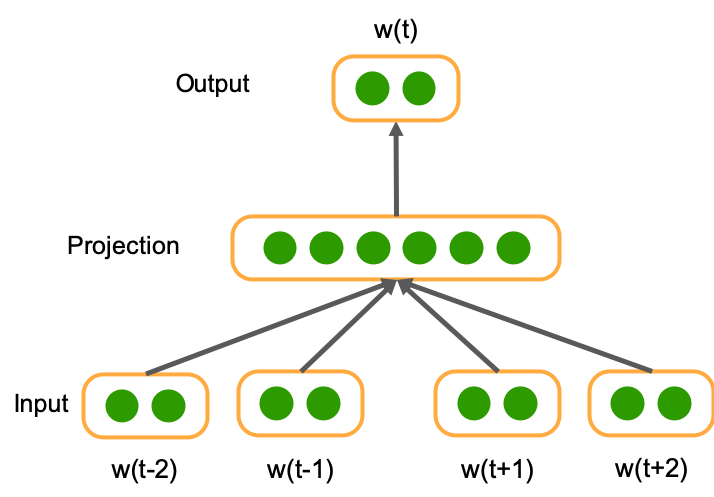
\includegraphics[height=4.3cm]{images/design/word2vec_cbow.png} \\
        (a) word2vec-CBOW
    \end{minipage}
    \begin{minipage}{0.48\textwidth}
        \centering
        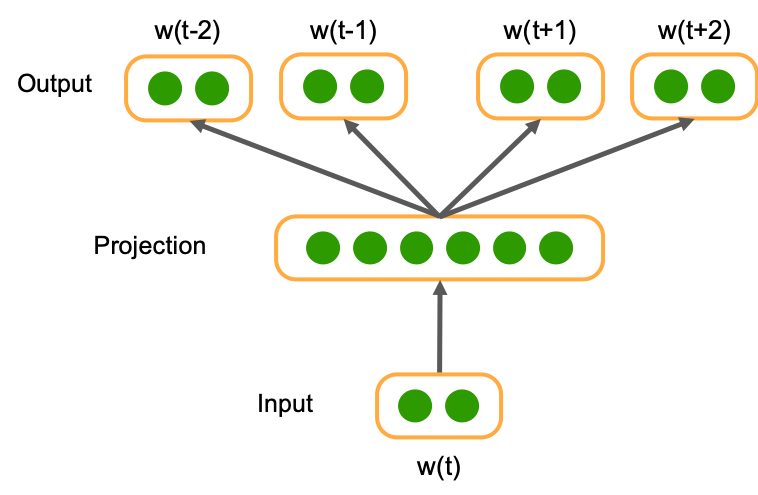
\includegraphics[height=4.3cm]{images/design/word2vec_sg.png} \\
        (b) word2vec-SG
    \end{minipage}
    \caption{Schematic for two Word Vector (word2vec) architectures}
    \label{fig:word2vec}
\end{figure}

\subsection{doc2vec}

To extend the embeddings to a higher level, the Paragraph Vector (doc2vec) is proposed to learn the representation for a variable-length of texts: sentence, paragraph and document. There are also two architectures within doc2vec, Paragraph Vector with Distributed Memory (PV-DM), corresponding to word2vec-CBOW, and Paragraph Vector with Distributed Bag-Of-Words (PV-DBOW), corresponding to word2vec-SG. As displayed in Figure \ref{fig:doc2vec}, both architectures introduce an additional document token that could be considered as the topic of each document (or in my framework, the mania level of transcript). The input in PV-DM is the concatenation of document vectors and word vectors, both of which are learned in the training process, but only the document vector is used for the inferring process. On the contrary, the PV-DBOW ignores the context words and predicts the words randomly sampled from the inferred document. It is obvious that PV-DBOW requires fewer data storage as it only saves softmax weights and PV-DM also needs to save the word vectors \cite{mikolov2014}. 

\begin{figure}[ht]
    \centering
    \begin{minipage}{0.55\textwidth}
        \centering
        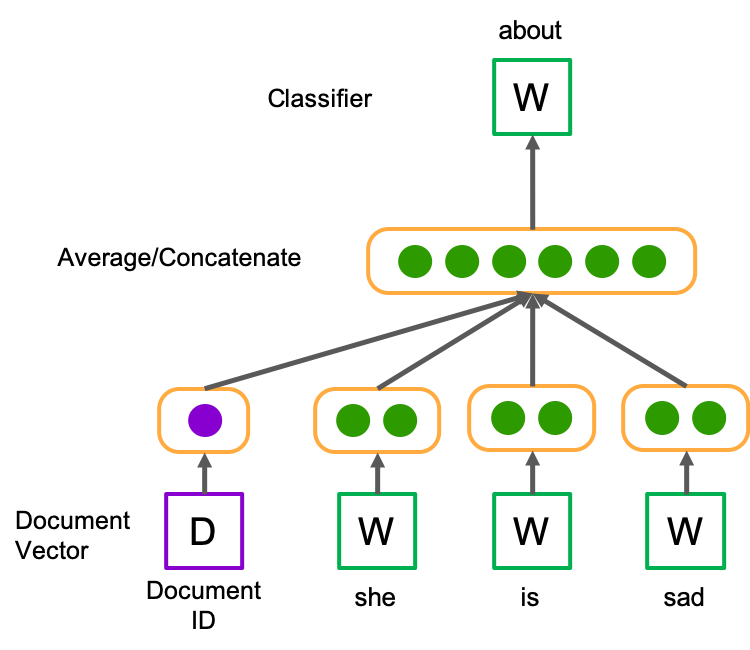
\includegraphics[height=5.4cm]{images/design/doc2vec_dm-m.png} \\
        (a) doc2vec-DM
    \end{minipage}
    \begin{minipage}{0.43\textwidth}
        \centering
        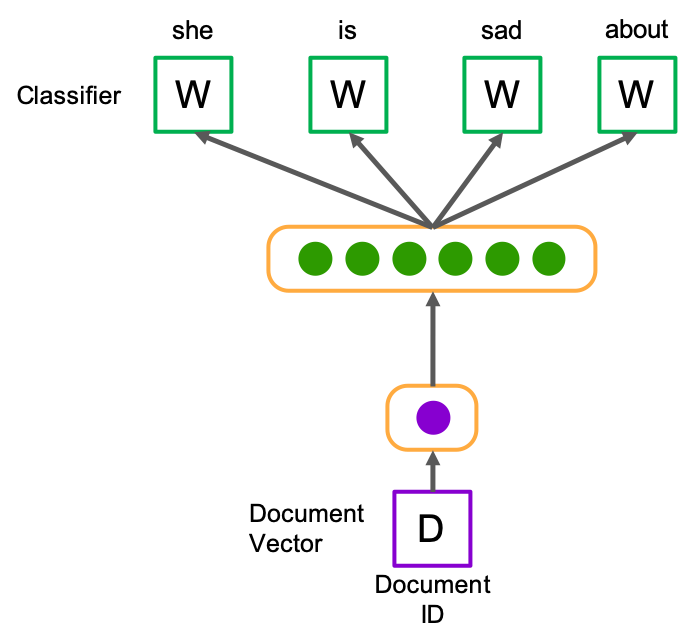
\includegraphics[height=5.4cm]{images/design/doc2vec_dbow.png} \\
        (b) doc2vec-DBOW
    \end{minipage}
    \caption{Schematic for two Paragraph Vector (doc2vec) architectures}
    \label{fig:doc2vec}
\end{figure}


\subsection{Implementation Details}
Some researchers have reported that PV-DBOW outperforms PV-DM in the sentiment analysis, contradictory results in the work of \cite{mikolov2014}. In addition, Yang \textit{et al.} only considers PV-DM architectures in their depression detection framework, and therefore, in my experiment, I investigate both PV-DM and PV-DBOW in the BD detection with different hyperparameter settings, as shown in Table \ref{tab:param_doc2vec}.


\begin{table}[ht]
    \centering
    \caption{Hyperparameter settings to investigate for document embedding}
    \begin{tabular}{l|l}
        \Xhline{2\arrayrulewidth}
        Hyperparameter & Values \\
        \hline
        model & \{PV-DM, PV-DBOW\} \\
        vector size & \{25, 50, 100\} \\
        window size & \{5, 10\} \\
        negative words & \{5, 10\} \\
        hierarchical softmax & \{0, 1\} \\
        \Xhline{2\arrayrulewidth}
    \end{tabular}
    \label{tab:param_doc2vec}
\end{table}

The translation of transcripts to English prior to the document embedding has been considered as it might help to understand the transcripts and to evaluate the embeddings. Nonetheless, I apply the doc2vec model directly on the Turkish transcripts to ensure the completeness of semantic content, which could be compromised in the translation, and after learning process, the document embeddings are evaluated with translation for better understanding. 

Due to the limited size of the BD corpus, I pre-train the doc2vec models on an external, large-scale Turkish corpus,``trwiki", to improve the performance of my models \cite{lau2016}. The ``trwiki" corpus is based on Wikimedia\footnote{\url{https://dumps.wikimedia.org/trwiki/}} dump service, which contains various kinds of texts in Turkish, such as articles, templates, media/file descriptions, and primary meta-pages. After training separate doc2vec models following the hyperparameter settings in Table \ref{tab:param_doc2vec}, I first evaluate their performance with a simple Random Forest (RF) classifier, the same classifier used in the baseline, and select the best-performing doc2vec model to infer the document vector for each transcript. These document vectors are used in the final fusion stage to predict the mania level of each session. In addition, visualizing the similar groupings of transcripts via Embedding Projector\footnote{\url{http://projector.tensorflow.org}} and the similar words stored in PV-DM models are presented to qualitatively examine the embedding space inferred by the doc2vec models.






\section{Multi-Task Learning}

In the context of Deep Learning, the generalization of the model could be improved if representations being shared across related tasks \cite{ruder2017}, and this approach is called Multi-Task Learning (MTL). There are two typical structures in MTL, hard parameter sharing and soft parameter sharing. Hard parameter sharing is applied by sharing the hidden layers between all tasks, with unchanged task-specific output layers (as shown in Figure \ref{fig:mtl}). Soft parameter sharing, on the other hand, separate all tasks with their own model and parameters (as shown in Figure \ref{fig:mtl}) with an objective to minimize the distance between parameters of different models.

\begin{figure}[ht]
    \centering
    \begin{minipage}[c]{0.42\textwidth}
    \centering
    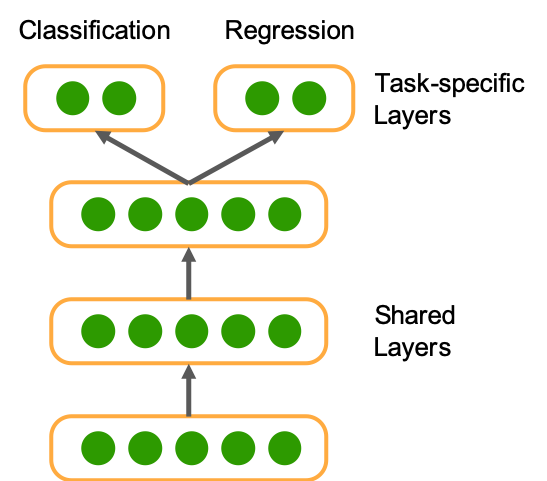
\includegraphics[height=4.2cm]{images/design/multitask_hard.png} \\
    (a) Hard parameter sharing
    \end{minipage}
    \begin{minipage}[c]{0.55\textwidth}
    \centering
    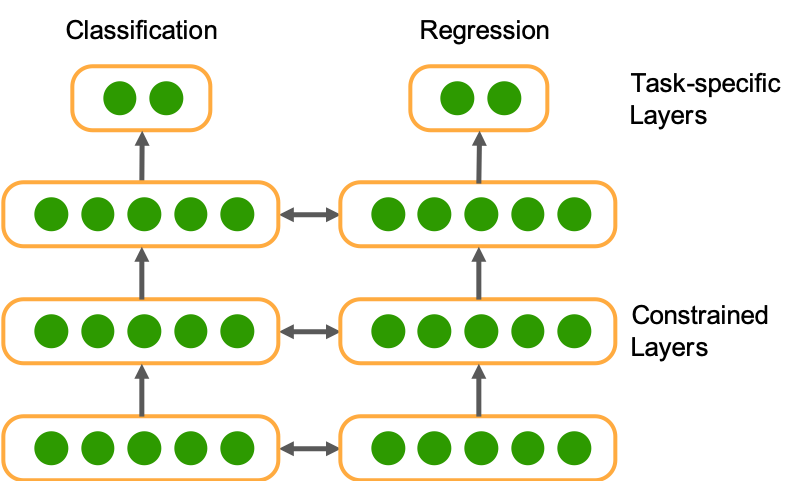
\includegraphics[height=4.2cm]{images/design/multitask_soft.png} \\
    (b) Soft parameter sharing
    \end{minipage}
    \caption{Schematic for two architectures in Multi-Task Learning frameworks}
    \label{fig:mtl}
\end{figure}

Hard parameter sharing architecture greatly reduces the risk of overfitting \cite{baxter1997} and more specifically, the risk of overfitting the shared parameters is an order N smaller than the risk of overfitting the task-specific parameters, where N which represents the number of tasks. I therefore adjust my deep neural network (DNN) classifier to learn on both classification task (mania levels) and regression task (YMRS scores). The joint loss function is defined as the weighted sum of cross entropy loss for classification and the Euclidean loss for regression, as shown in Equation \ref{eq:multi_loss}.

\begin{equation} 
\begin{split}
 \mathcal{L} & = \mathcal{W}_c \mathcal{L}_c + \mathcal{W}_r \mathcal{L}_r \\
             & = \mathcal{W}_c (-\sum_{c=1}^N y_c \log(p_c)) + \mathcal{W}_r (\frac{1}{M} \sum_{i=1}^M \parallel y_r - p_r \parallel ^ 2)
\end{split}
\label{eq:multi_loss}
\end{equation}

where $\mathcal{W}_c$ and $\mathcal{W}_r$ represent the weight for two losses, $y_c$ and $y_r$ are values for two tasks while $p_c$ and $p_r$ are the predicted values, and $N$ is the number of classes and $M$ is the number of samples in the training set.
